The system is controlled by five keys on a PS/2-connected keyboard. Down in the table you can see which key that changes what in the system.


\begin{figure}[h]
\centering
%\caption{PS/2 keys and how the input affects the system.}
\begin{tabular}{|c|c|}
\hline
KEY & Function\\ \hline
U ARROW & Volume Increase\\ \hline
L ARROW & Balance Bias Left\\ \hline
D ARROW &  Volume Decrease\\ \hline
R ARROW &  Balance Bias Right\\ \hline
END		&  Mute Volume\\ \hline
\end{tabular}
\caption{PS/2 keys and how the input affects the system.}
\label{fig:scancodes}
\end{figure}


The volume level has eleven different stages, exclusive mute. When the volume is at max, the whole bar will be red, and when the volume is decreased by one the bar will decrease to show the current volume.

The balance level has eighteen different stages. Eight for left balance, eight for right balance and one stage when the signal is equal. When the balance is equal for left and right the only thing you will notice is the bar and divider. But when you for example press the left arrow, the left side will be filled and the outgoing volume on the right will decrease.

To indicate that mute is enabled you can see a green speaker with a cross to the left side of the picture, and when mute is disabled there will only be a black fiel. Apparent is that the "after" bars will not show anything, due to nothing is being sent out. 

You will be able to see one peak level indicator for each bar, the peak level indicator falls slowly when the power bar is lower than the peak level indicator. With our peak level indicator our user experience is taken to a whole new level, as you will notice when you use our system you will be overwhelmed by the effect.

\begin{figure}[h]
	\centering
        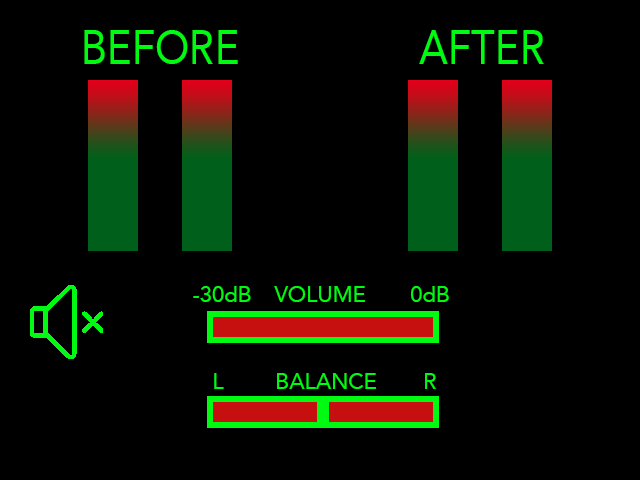
\includegraphics[scale=1]{UI2.png}
       \caption{User interface}
        \label{fig:user interface}
\end{figure}


